
\chapter{Một số kiến thức cơ sở}

\indent Mục đích chính của luận văn này là về phương pháp tiếp cận sử dụng hàm Lambert W để nghiên cứu các hệ điều khiển có trễ. Trong chương này chúng ta sẽ trình bày phần kiến thức chuẩn bị cho Chương 2, bao gồm hai mục chính (1) giới thiệu sơ lược về hàm Lambert W, và (2) nhắc lại một số tính chất cơ bản của các hệ điều khiển không trễ.


\section{Sơ lược về hàm Lambert W}\label{sec1.1}

Theo định nghĩa \cite{Cor96,Eul77,Lam58}, mọi hàm $W(s)$ thỏa mãn:
\begin{equation}\label{2}
 W(s)e^{W(s)}=s
\end{equation}
được gọi là hàm Lambert W. Hàm Lambert W, với đối số phức $s$, là một hàm có giá trị phức với vô hạn nhánh, $k=0,\pm 1,\pm 2,...,\pm\infty$. Hàm vô hướng Lambert W đã được lập trình sẵn trong nhiều phần mềm tính toán khoa học, ví dụ như hàm \emph{lambertw} trong MATLAB. Hàm ma trận Lambert W \cite{Yi10} có thể thu được bằng cách sử dụng phép biến đổi tương tự và có thể dễ dàng đánh giá bằng cách sử dụng gói công cụ LambertWDDE \cite{Dua10}.
Các hàm số này rất hữu ích trong nghiên cứu tổ hợp (ví dụ như phép liệt kê của cây) cũng như trong thuyết tương đối và cơ học lượng tử. 
Chúng có thể được sử dụng để giải rất nhiều phương trình khác nhau có chứa đến số mũ (ví dụ như cực đại của các phân phối Planck, Bose-Einstein và Fermi-Dirac) cũng như trong việc giải các phương trình vi phân có trễ như sẽ thảo luận trong chương tiếp theo.

\subsection{Hàm Lambert vô hướng}       
Hàm Lambert $W$ được định nghĩa là một hàm phức ngược đa trị của hàm $w \mapsto we^{w}$ với $w \in \mathbb{C}$. Năm 1758, Lambert nghiên cứu phương trình $x = q + x^{m}$ với ẩn số x. Trong \cite{Eul77}, Euler biến đổi phương trình Lambert về dạng đối xứng hơn 
%
\begin{align} x^{\alpha} - x^{\beta} = (\alpha - \beta)vx^{\alpha + \beta} \end{align}
%
bởi thay thế $x = x^{-\beta}$ và đặt $m = \frac{\alpha}{\beta}$ và $q = (\alpha - \beta)v$.
Phiên bản Euler của chuỗi Lambert có dạng sau 
\begin{align}
\begin{split}
x^{\gamma} = 1 + \gamma v + \frac{1}{2}\gamma(\gamma + \alpha + \beta)v^{2} + \frac{1}{6}\gamma(\gamma + \alpha + 2\beta)(\gamma + 2\alpha + \beta)v^{3} \\ + \frac{1}{24}\gamma(\gamma + \alpha + 3\beta)(\gamma + 2\alpha + 2\beta)(\gamma + 3\alpha + \beta)v^{4} + ...
\end{split}.
\end{align}
Sau khi chuyển đổi chuỗi, Euler nhìn vào trường hợp đặc biệt, bắt đầu từ $\alpha = \beta$. Để nhìn thấy ý tưởng từ phương trình ban đầu, ta chia (1.1) cho $(\alpha - \beta)$ và cho $\beta \rightarrow \alpha$, ta được
%
\begin{align*}
\displaystyle \lim_{\beta \to \alpha}\frac{x^{\alpha}-x^{\beta}}{\alpha - \beta} = vx^{2\alpha}.
\end{align*}
%
Do đó
%
\[
x^{\alpha}\log \alpha = vx^{2\alpha}.
\]
%
Vì vậy
\[
\log x = vx^{\alpha} \ .
\]
%
Euler chú ý rằng nếu ta giải được phương trình (1.3) với $\alpha = 1$ thì ta có thể giải được nó với mọi $\alpha \neq 0$. Để thấy điều này, ta nhân phương trình (1.3) với $\alpha$, dẫn đến $\alpha \log x = \log x^{\alpha}$. Đặt $z = x^{\alpha}$ và $u = \alpha v$, ta có $\log z = u z$ là kết quả của phương trình (1.3) với $\alpha = 1$. \\

Để giải phương trình (1.2), đầu tiên Euler cho $\alpha = \beta = 1$ và viết lại (1.2) dưới dạng chuỗi của $\frac{x^{\gamma}-1}{\gamma}$. Từ phương trình (1.2) thì 
\begin{align*}
\frac{x^{\gamma}-1}{\gamma} = v + \frac{1}{2}(\gamma+2)v^{2} + \frac{1}{6}(\gamma+3)(\gamma+3)v^{3} + ... 
\end{align*}
Tiếp đến, ông cho $\gamma \rightarrow$ 0, vì 
%
\begin{align*} 
\displaystyle \lim_{\gamma \to 0}\frac{x^{\gamma}-1}{\gamma} = \log x 
\end{align*}
%
nên ta thu được
%
\begin{align} 
\log x = v + \frac{2^{1}}{2!}v^{2} + \frac{3^{2}}{3!}v^{3} + \frac{4^3}{4!}v^{4} + ... 
\end{align}
Chuỗi bên vế phải hội tụ với mọi $|v| < \dfrac{1}{e}$, và nó được định nghĩa là hàm $T(v)$ và được gọi là hàm cây \cite{Cor96}. Nó có giá trị bằng với $-W(-v)$ với $W(z)$ được định nghĩa là hàm thỏa mãn 
%
\begin{equation}\label{eq1}
W(z)e^{W(z)} = z.
\end{equation} 
%
Ta sẽ gọi tắt 2 hàm này là $T$ và $W$. Hai hàm này được sử dụng trong rất nhiều ứng dụng, xem \cite{Cor96}. 
%
Bởi vì ánh xạ $x \mapsto xe^x$ không phải là đơn ánh nên $W(z)$ không xác định duy nhất từ phương trình \eqref{eq1}. 
Trong thực tế hàm Lambert $W$ là hàm có giá trị phức đối với đối số phức $z$ và nó có vô hạn nhánh $W_{k}$, ở đó $k = -\infty, ..., -1, 0 , 1, ..., \infty$. 
Như có thể thấy trong Hình \ref{fig1}, hàm Lambert W có hai nhánh thực với điểm nhánh là $(-e^{-1},-1)$. 
Nhánh dưới, $W_{-1}(z)$, xác định trên đoạn $[-e^{-1}, \ 0]$, còn nhánh trên, $W_{0}(z)$, xác định trên đoạn $[-e^{-1}, \ \infty)$.
Ngoại trừ điểm $z=-e^{-1}$ mà nhánh chính $W_0$ không khả vi tại đó, tất cả các nhánh đều là giải tích địa phương. Nhánh chính và tất cả các nhánh khác của hàm Lambert có thể được tính toán giải tích thông qua việc tính toán chuỗi. Các ngôn ngữ tính toán khoa học phổ biến hiện nay như Python, Matlab, Maple, Mathematica, ... đều có hàm Lambert (vô hướng) dựng sẵn với độ chính xác tùy ý.
%\begin{verbatim}
%syms x
%fplot(lambertw(x))
%hold on
%fplot(lambertw(-1,x))
%hold off
%axis([-0.5 4 -4 2])
%title('Hàm Lambert W , 2 nhánh chính')
%legend('k=0','k=-1','Location','best')
%\end{verbatim}

\begin{figure}[h]
	\centering
	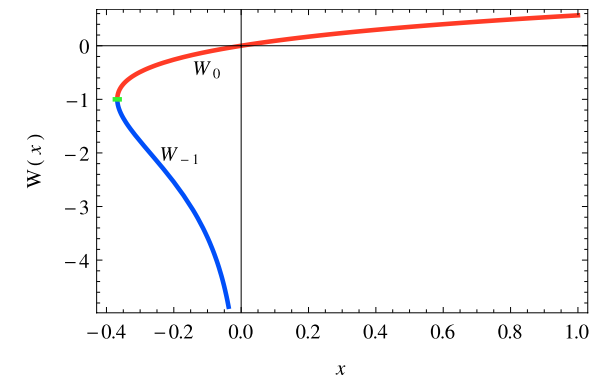
\includegraphics[scale=0.7]{hinh/Screenshot_1}
	\caption{Hàm Lambert với 2 nhánh chính k=0, k=-1}
	\label{fig1}
\end{figure}

\subsection{Dạng ma trận  của hàm Lambert}\label{sec1.1.2}
Nhắc lại rằng với $z\in \mathbb{C}$, hàm Lambert W được định nghĩa là một hàm ngược đa trị của hàm vô hướng $z\mapsto ze^z$
$$W_k(z)\in\{w\in\mathbb{C}:z=we^w\}$$
trong đó $W_k$ là nhánh thứ $k$, $k\in\mathbb{Z}$.  Bây giờ ta sẽ đi xây dựng khái niệm hàm Lambert W cho ma trận. Đầu tiên ta định nghĩa hàm Lambert W cho ma trận theo dạng chuẩn tắc Jordan
$$ J=\text{diag}(J_{n_1}(\lambda_1),J_{n_2}(\lambda_2),\cdots,J_{n_s}(\lambda_s))$$
với $J_n(\lambda)$ là ma trận Jordan cỡ $n\times n$ tương ứng với giá trị riêng $\lambda$ bội $n$. Vậy:
$$W_k(J)=\text{diag}(W_{k_1}(J_{n_1}(\lambda_1)),W_{k_2}(J_{n_2}(\lambda_2)),\cdots,W_{k_s}(J_{n_s}(\lambda_s))).$$
Chú ý rằng ta có thể lấy các nhánh khác nhau cho mỗi khối Jordan. Nếu $J$ có $s$ khối Jordan và tập chỉ số cho các nhánh của hàm Lambert W là $\mathbb{Z}$ thì tập chỉ số của các nhánh $W_k(j)$ là $\mathbb{Z}^s$. 
Với khối Jordan có số chiều là 1 thì ta có thể sử dụng hàm Lambert vô hướng. Với khối có số chiều lớn hơn, ta sẽ định nghĩa hàm Lambert W (với nhánh cố định) của một khối Jordan bởi định nghĩa tiêu chuẩn của hàm ma trận dạng
$$P(J_k(\lambda))=\begin{bmatrix}
p(\lambda)&p^\prime(\lambda)&\cdots & \dfrac{1}{(k-1)!}p^{(k-1)}(\lambda)\\
& p(\lambda) & \ddots & \vdots\\
 & & \ddots & p^\prime(\lambda)\\
& &  & p(\lambda)
\end{bmatrix}
\ . 
$$
Do đó 
$$ W_k(J_n(\lambda))=\begin{bmatrix}
W_k(\lambda)&W_k^\prime(\lambda)&\cdots & \dfrac{1}{(n-1)!}W_k^{(n-1)}(\lambda)\\
& W_k(\lambda) & \ddots & \vdots\\
 & & \ddots & W_k^\prime(\lambda)\\
& &  & W_k(\lambda)
\end{bmatrix}
\ .
$$
Nếu $k=0$ thì ta phải giả sử thêm là $\lambda\neq -e^{-1}$ (vì $W_0^\prime(-e^{-1})$ không xác định).\\
Bên cạnh đó chúng ta chú ý rằng bằng cách lấy đạo hàm cả hai vế của đẳng thức $x = W(x) e^{W(x)}$ ta có
%

\begin{equation}\label{der-w}
W'(x) = \dfrac{1}{x+e^{W(x)}} = \dfrac{W(x)}{x \ (1+W(x))} \ .
\end{equation}
%
Ta hoàn thành việc định nghĩa hàm Lambert W cho ma trận bằng việc biến đổi ma trận về dạng chuẩn tắc Jordan $A=SJS^{-1}$. Từ đó ta có thể định nghĩa 
$$W_k(A)=SW_k(J)S^{-1}.$$
Khi đó với mọi $k$ ta có
%
\begin{align*}
W_k(A) \ e^{W_k(A)} &= S W_k (J) S^{-1} \ S e^{W_k (J)} S^{-1} \\
&= S J S^{-1} = A.
\end{align*}
%
Chú ý rằng với nhánh chính $k=0$, từ bây giờ ta sẽ giả sử rằng $-e^{-1}$ không phải là giá trị riêng tương ứng với khối Jordan với số chiều lớn hơn 1, tức là
$$\text{rank}(A+e^{-1}I)=\text{rank}(A+e^{-1}I)^2.$$

\begin{vd}\label{vd1.1}
Trong ví dụ này chúng ta sẽ minh họa cho việc xác định hàm Lambert của một ma trận. Xét ma trận
%
\[
A = \m{1 & 1 & 1 \\ 0 & 1 & 2 \\ 0 &  0  &  3}. 
\]
%
Phân tích Jordan của ma trận A là $A = S J S^{-1}$, trong đó
%
\[
S = \m{ 1 &  -2 & -1 \\ 1 &    0  &  -2 \\ 	1  &   0  &   0 }, \quad J = \m{3 &  0 & 0 \\ 0 &  1 &  1 \\ 0 &  0 & 1} \ .
\]
%
Nếu ta chọn $k_1  = 0$, $k_2 = 2$ tương ứng với hai block Jordan, khi đó ta có 
%
\[
W_k(A) = S \m{W_0(3) & 0  \\ 0  & W_2\left( \m{1 &  1 \\ 0 &  1} \right) } S^{-1} 
 = S \m{W_0(3) & 0 & 0 \\ 0  & W_2(1) & W'_2(1) \\  0 & 0  & W_2(1)} S^{-1} \ .
\]
%
Do đó, bằng việc tính toán $ W'_2(1) $ dựa trên công thức \eqref{der-w} ta có
%
\[
W_k(A) = S \m{1.0499 & 0 & 0 \\ 0 & -2.4016 +10.7763i &  1.0119 + 0.0913i \\ 0 & 0 & -2.4016 +10.7763i} S^{-1} \ .
\]
%
\end{vd}

\section{Một số tính chất cơ bản của các hệ điều khiển không trễ}\label{sec1.2}

Xét một hệ điều khiển không trễ dạng
%
\begin{equation}\label{1}
\begin{split}
\dot{x}(t) &= Ax(t)+Bu(t), \\
y(t) &= Cx(t) + Du(t),
\end{split}
\end{equation}
%
trong đó các ma trận hệ số là $A \in \R^{n,n}$, $B\in \R^{n,p}$, $C\in \R^{m,n}$, $D\in \R^{m,p}$. \ 
Công thức nghiệm $x(t)$ của hệ \eqref{1} là
%
\begin{equation}\label{sol}
x(t) = e^{At} x(0) + \int_{0}^{t} e^{A(t-s)} B u(s) ds \ .
\end{equation}
%
Bởi vì hệ phương trình vi phân thường $\dot{x}(t) = Ax(t)$ có phổ hữu hạn, tính ổn định của hệ có thể được xác định bằng cách kiểm tra các vị trí của một số hữu hạn các giá trị riêng trong mặt phẳng phức. \
Bên cạnh đó, các khái niệm cơ bản khác trong lý thuyết điều khiển của hệ thống tuyến tính (không trễ) sẽ được trình bày trong hai định nghĩa sau đây.
%
\begin{dng}\citep{Che98}
i) Hệ điều khiển \eqref{1} hay cặp $(A,B)$ được gọi là \emph{điều khiển được} nếu với mọi trạng thái ban đầu $x(0)=x_0$ và trạng thái cuối $x_1$, tồn tại một hàm điều khiển để truyền từ trạng thái $x_0$ sang trạng thái $x_1$ trong thời gian hữu hạn $t_1>0$, tức là $x(t_1) = x_1$. \\
ii) Hệ điều khiển \eqref{1} hay cặp $(A,C)$ được gọi là \emph{quan sát được} nếu với mọi trạng thái ban đầu $x(0)=x_0$ chưa biết, tồn tại một thời điểm $t_1 > 0$ sao cho $x_0$ có thể được xác định duy nhất dựa trên hàm điều khiển $u(t)$ và hàm đầu ra $y(t)$ trên đoạn $[0,t_1]$. 
\end{dng}
%

\begin{dng}\citep{Che98} Xét hệ điều khiển \eqref{1}. Khi đó các ma trận 
%
\[
W_c(t) : = \int_{0}^{t} e^{A(t-s)} B B^T e^{A^T (t-s)}ds
\]
%	
và 
%
\[
W_o(t) : = \int_{0}^{t} e^{A^T(t-s)} C^T C  e^{A (t-s)}ds
\]
%	
lần lượt được gọi là \emph{ma trận điều khiển Gramian} và \emph{ma trận quan sát Gramian}.
\end{dng}

Trong hai định lý sau chúng ta sẽ nhắc lại các điều kiện cần và đủ để kiếm tra 
tính điều khiển được và tính quan sát được của hệ \eqref{1}.

\begin{dly}\citep[Chương 6]{Che98}
Hệ \eqref{1} là điều khiển được khi và chỉ khi một trong những điều kiện tương đương sau được thỏa mãn.
\begin{enumerate}
\item[i)] Ma trận điều khiển Gramian $W_c(t)$ là khả nghịch với mọi $t>0$. 
\item[ii)] Ma trận điều khiển được \ $\cC := \m{B & AB & A^2B & \dots & A^{n-1} B}$ \ là đủ hạng dòng.
\item[iii)] Ma trận $\m{A-\lb I_n & B}$ là đủ hạng dòng với mọi $\lb \in \mathbb{C}$.
\end{enumerate}
\end{dly}


\begin{dly}\citep[Chương 6]{Che98}
	Hệ \eqref{1} là quan sát được khi và chỉ khi một trong những điều kiện tương đương sau được thỏa mãn.
	\begin{enumerate}
		\item[i)] Ma trận quan sát Gramian $W_o(t)$ là khả nghịch với mọi $t>0$. 
		\item[ii)] Ma trận quan sát được \ $\mathcal{O} := \m{C^T & \left( CA \right) ^T & \dots & \left( CA^{n-1}\right) ^T }$ \ 
		là đủ hạng dòng.
		\item[iii)] Ma trận $\m{A-\lb I_n \\ C}$ là đủ hạng dòng với mọi $\lb \in \mathbb{C}$.
	\end{enumerate}
\end{dly}

\begin{dly}\cite[Chương 8]{Che98} Xét hệ điều khiển \eqref{1}. Khi đó ta có các khẳng định sau. \\
i) Cặp $(A-BK,B)$, với ma trận $K$ bất kỳ thuộc $\R^{p,n}$, là điều khiển được khi và chỉ khi cặp $(A,B)$ là điều khiển được. \\
ii) Tất cả các giá trị riêng của ma trận $A-BK$ có thể chọn được bất kỳ (nếu như các giá trị riêng phức liên hợp đi thành đôi một) bằng cách lựa chọn một ma trận điều khiển phản hồi $K \in \R^{p,n}$ phù hợp khi và chỉ khi cặp $(A,B)$ là điều khiển được.
\end{dly}

Nếu hệ đã cho là điều khiển được thì một bộ (thiết bị) điều khiển (controller) đóng kín có thể được thiết kế bằng nhiều phương pháp, bao gồm cả điều khiển phản hồi và phương pháp thiết kế giá trị riêng (eigenvalue assignment). Tương tự, nếu một hệ có thể quan sát được, sau đó, một bộ quan sát (observer) hay bộ ước lượng trạng thái (state estimator) cũng có thể được thiết kế bằng cách sử dụng phương pháp thiết kế giá trị riêng. Chi tiết độc giả quan tâm có thể tham khảo trong \citep[Chương 8, 9]{Che98}. 





















